\section{Introduction}
\label{sec:intro}

Reinforcement learning with verifiable rewards (RLVR) trains large language models on tasks whose outputs can be automatically checked, such as code against test suites or mathematical reasoning against ground-truth answers \citep{le2022coderl,shao2024deepseekmath,guo2025deepseekr1}. The verifier provides a response-level reward to an output that may span hundreds or thousands of tokens.

On-policy distillation (OPD) provides denser supervision by training the student on its own rollouts using token-level targets from a teacher model~\citep{agarwal2024opd}. On-policy self-distillation (OPSD) removes the need for a distinct teacher: the {teacher} is the same model with additional privileged context unavailable to the student, such as a code execution trace, correct rollout, or ground-truth solution~\citep{hubotter2026sdpo,zhao2026sdr,song2026rltf}. The student then minimizes the divergence from the teacher at each token.

In standard OPSD, teacher targets are evaluated at prefixes in student-sampled trajectories. When the teacher favors a different token at a given prefix, its target can teach the student to prefer that token, while the collected suffix follows the original student choice. Supervising the continuation \textit{after} the teacher-preferred alternative requires collecting its successor contexts. This creates a training-time data-collection bottleneck: standard OPSD provides direct teacher supervision at subsequent prefixes on an alternative branch only when those prefixes appear in student-sampled rollouts.

Teacher-generated trajectories offer another way to expose alternative continuations. TRD~\citep{jiang2026trajectory} uses a privileged-context teacher to rewrite student responses. The student is then trained on continuations generated by a teacher with access to information unavailable to the student at deployment. In SciKnowEval, TRD exhibits late-training accuracy collapse as responses reach the generation limit (Section~\ref{sec:method-student-generation}). This failure case motivates using the teacher to select a branch action and the student to generate the continuation.

Our insight is to use teacher--student disagreement to identify where to branch and collect an alternative student-generated continuation for supervision. We first analyze where disagreement concentrates, then test its value for trajectory steering through controlled token interventions (Section~\ref{sec:analysis}). On failed LiveCodeBench rollouts, the peak-disagreement position $\tstar$ accounts for $9$--$20\%$ of total response KL divergence across model scales, identifying a concentrated target for intervention. 
On these failed rollouts, Qwen3-8B achieves $9.9\%$ continuation success when the teacher-preferred token is forced at $\tstar$, compared with $1.7\%$ when the original token is retained, with the student regenerating the suffix in both cases.
This result motivates using a single teacher-selected action to collect alternative student continuations for dense supervision within the same training iteration.

We turn this insight into \textbf{Trajectory-Intervention Self-Distillation~(\method{})}, a branch--regenerate--distill framework (Figure~\ref{fig:overview}). For each eligible failed rollout, \method{} finds the peak-divergence position $\tstar$, forces the teacher's preferred token, and lets the student regenerate the suffix. It then distills teacher predictions along the full trajectory, including the original student prefix, the intervened token, and the regenerated student suffix. This supervises both the branch decision and subsequent predictions at the newly visited prefixes.

{\method{} improves Avg@4 over SDPO by 1.2 percentage points on average across three coding models. Across the four science domains, \method{} improves Avg@128 over SDPO by an average of 0.8 points under equal training steps and 0.3 points under equal training time (Section~\ref{sec:experiments}). These results demonstrate the benefit of teacher-guided branching both with and without rich execution feedback.}



Our contributions are:
\begin{itemize}[itemsep=0pt, topsep=0pt, parsep=0pt, partopsep=0pt, leftmargin=*]
\item A diagnostic framework that distinguishes local correction from trajectory steering through controlled token interventions. We show that direct token substitution rarely repairs failed responses, whereas teacher-guided branching at peak disagreement improves Qwen3-8B continuation success (Section~\ref{sec:analysis}).
\item \textbf{\method{}}, a simple self-distillation method that forces a teacher-preferred token, lets the student regenerate the suffix, and distills teacher predictions along the resulting trajectory. This makes teacher supervision available along alternative continuations without waiting for the student to select the branch on its own (Section~\ref{sec:method}).
\item {An evaluation across coding and science showing higher average performance than SDPO under the reported step- and time-based comparisons (Section~\ref{sec:experiments}).}

\end{itemize}


\begin{figure*}[t]
  \centering
  \begin{minipage}[t]{\textwidth}
    \centering
    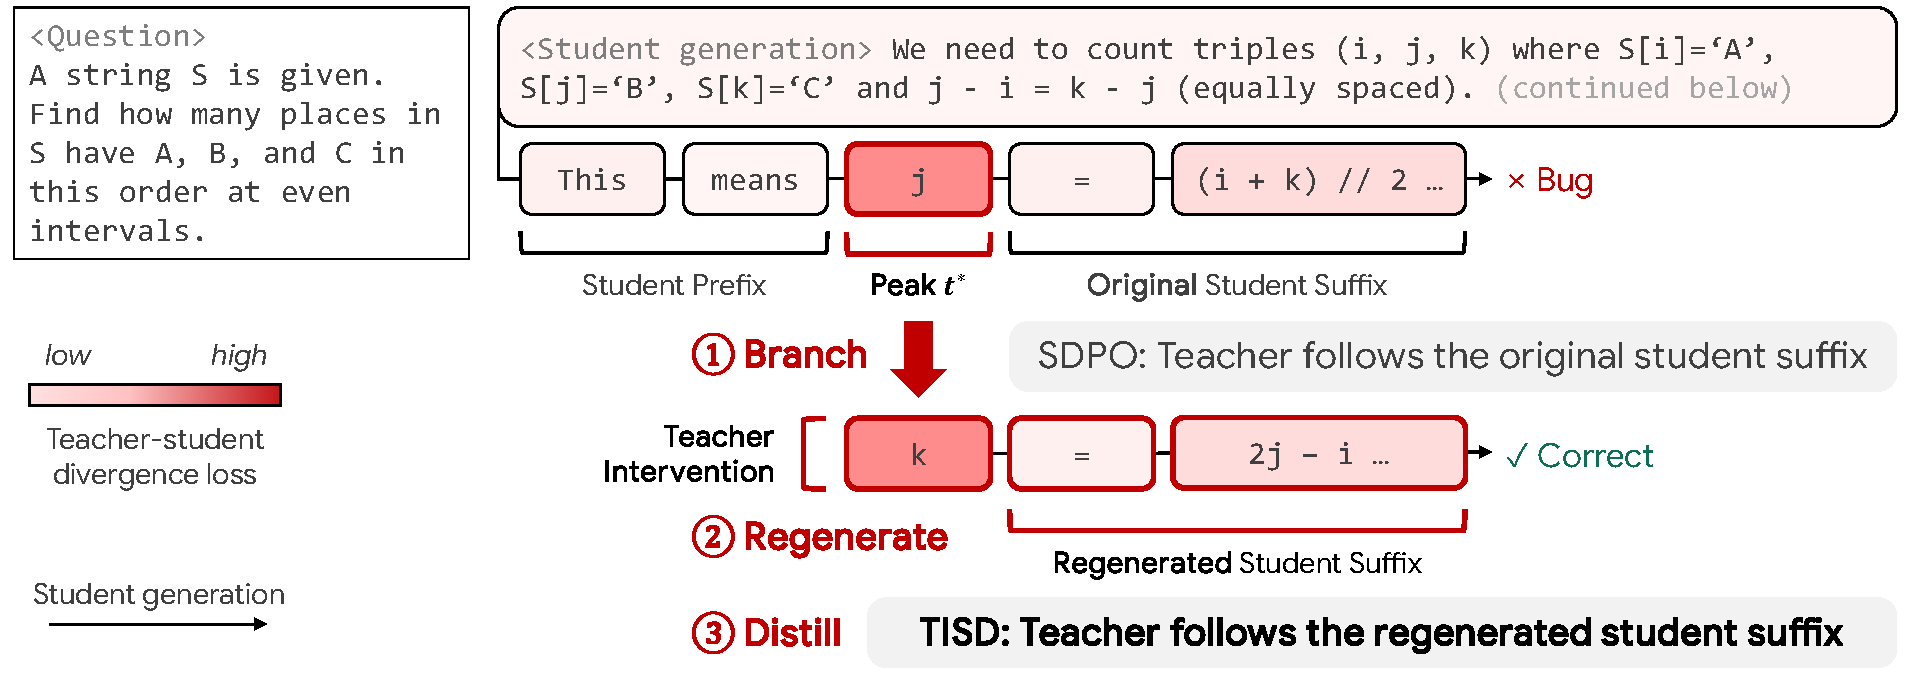
\includegraphics[width=\linewidth]{figures/overview.pdf}

\captionsetup{skip=3pt}
\captionof{figure}{\method{} changes where self-distillation is evaluated. Standard OPSD (e.g., SDPO) distills teacher targets along the original student trajectory, including the suffix that follows the student's sampled action. \method{} instead forces the teacher-preferred token at the peak-divergence position, lets the student regenerate the suffix, and distills the resulting trajectory. This exposes successor prefixes that are absent from the original rollout. }
    \label{fig:overview}
  \end{minipage}
  \vspace{-0.2cm}
\end{figure*}
